\section{选题背景及研究现状}

\subsection{选题背景}
\begin{frame}{\insertsubsection}
	\begin{center}
		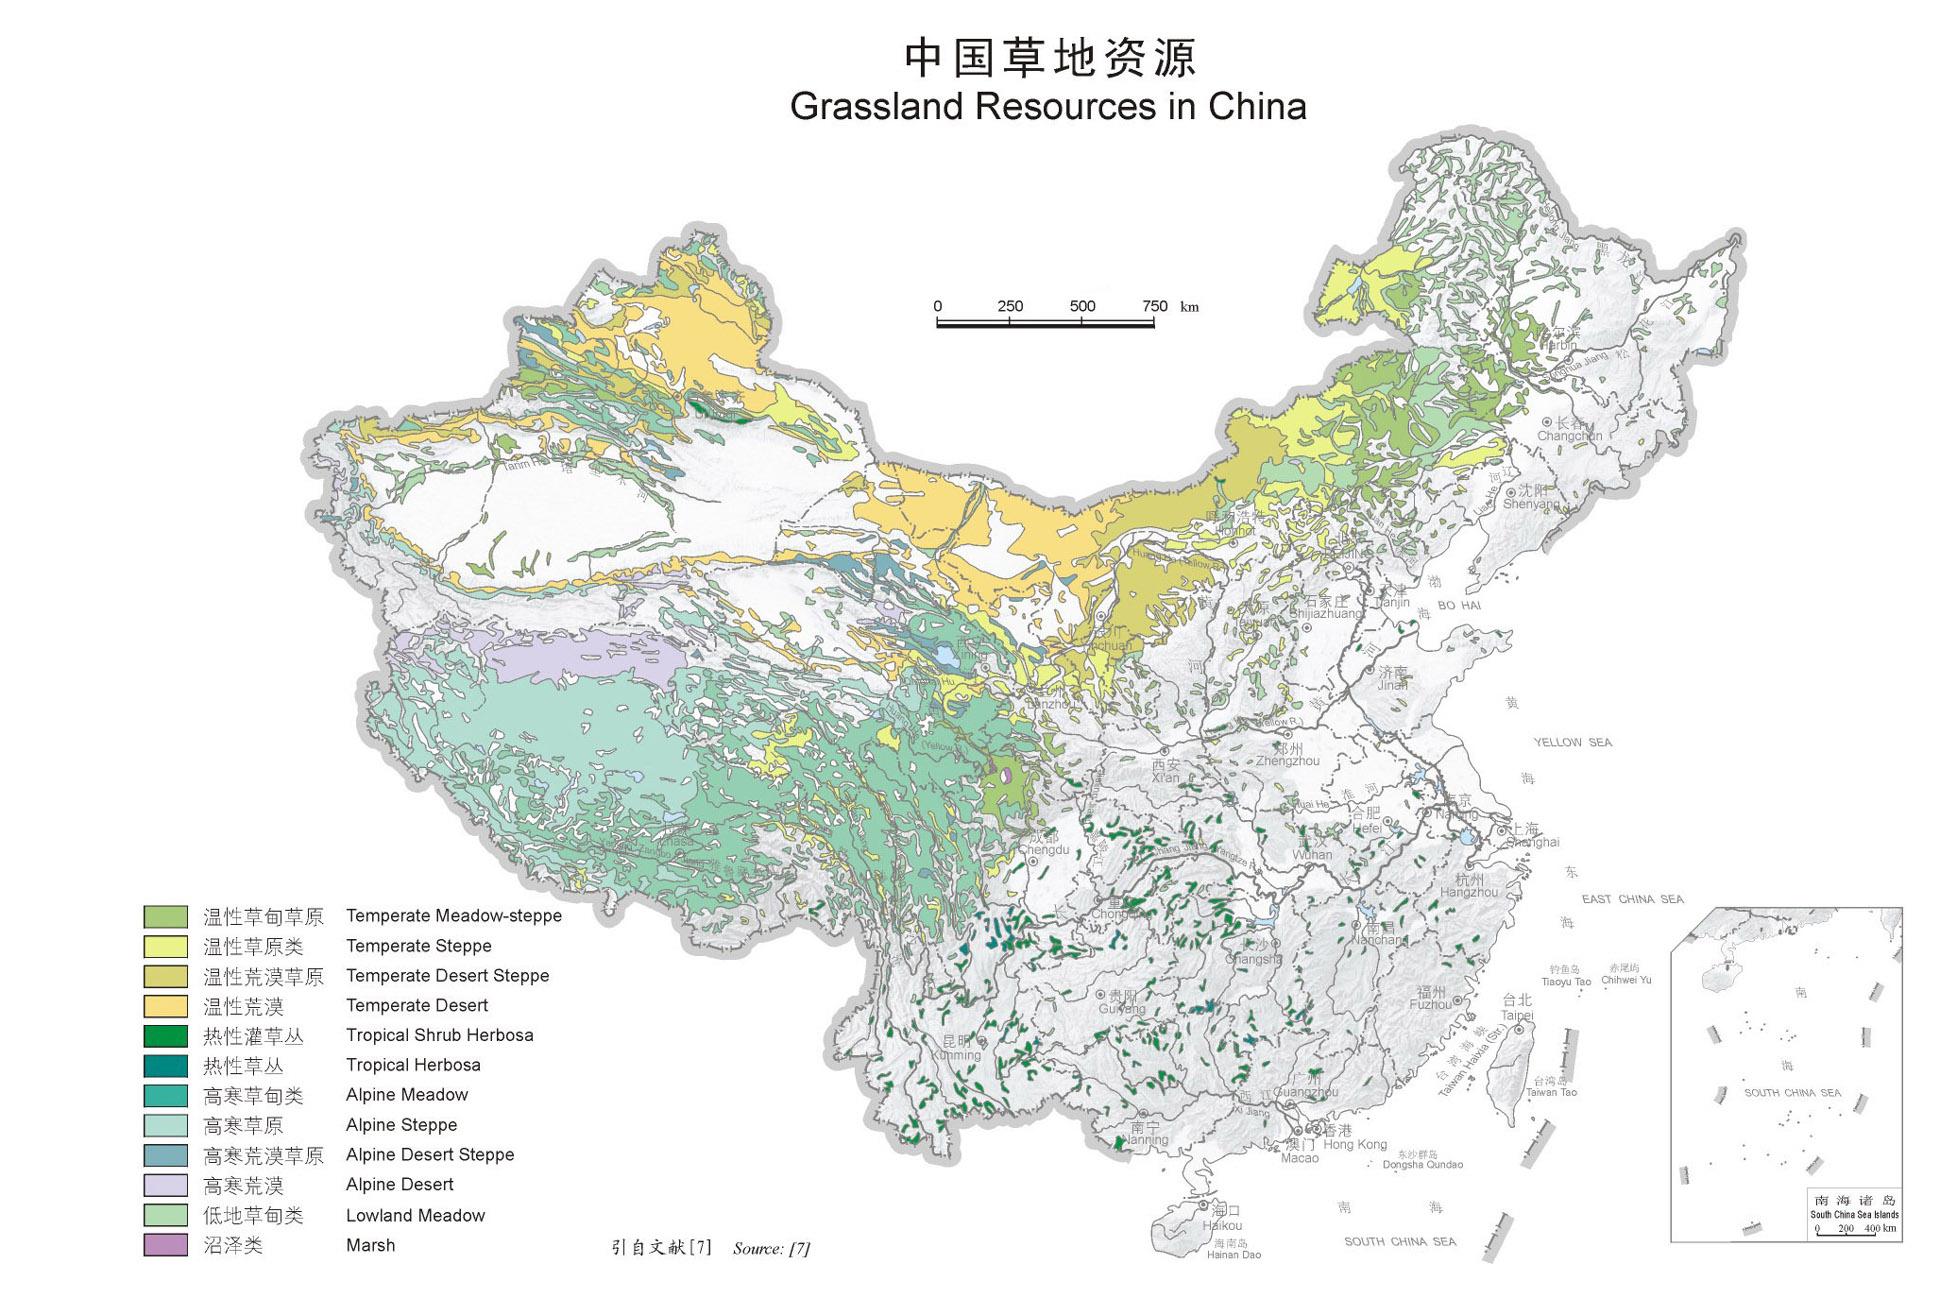
\includegraphics[width = 0.9\textwidth]{./pic/1.1.1.jpg}
	\end{center}
\end{frame}
\begin{frame}{\insertsubsection}
	\begin{columns}
		\column{0.7\textwidth}
		\hskip 15ex 中国草地资源
		\begin{center}
			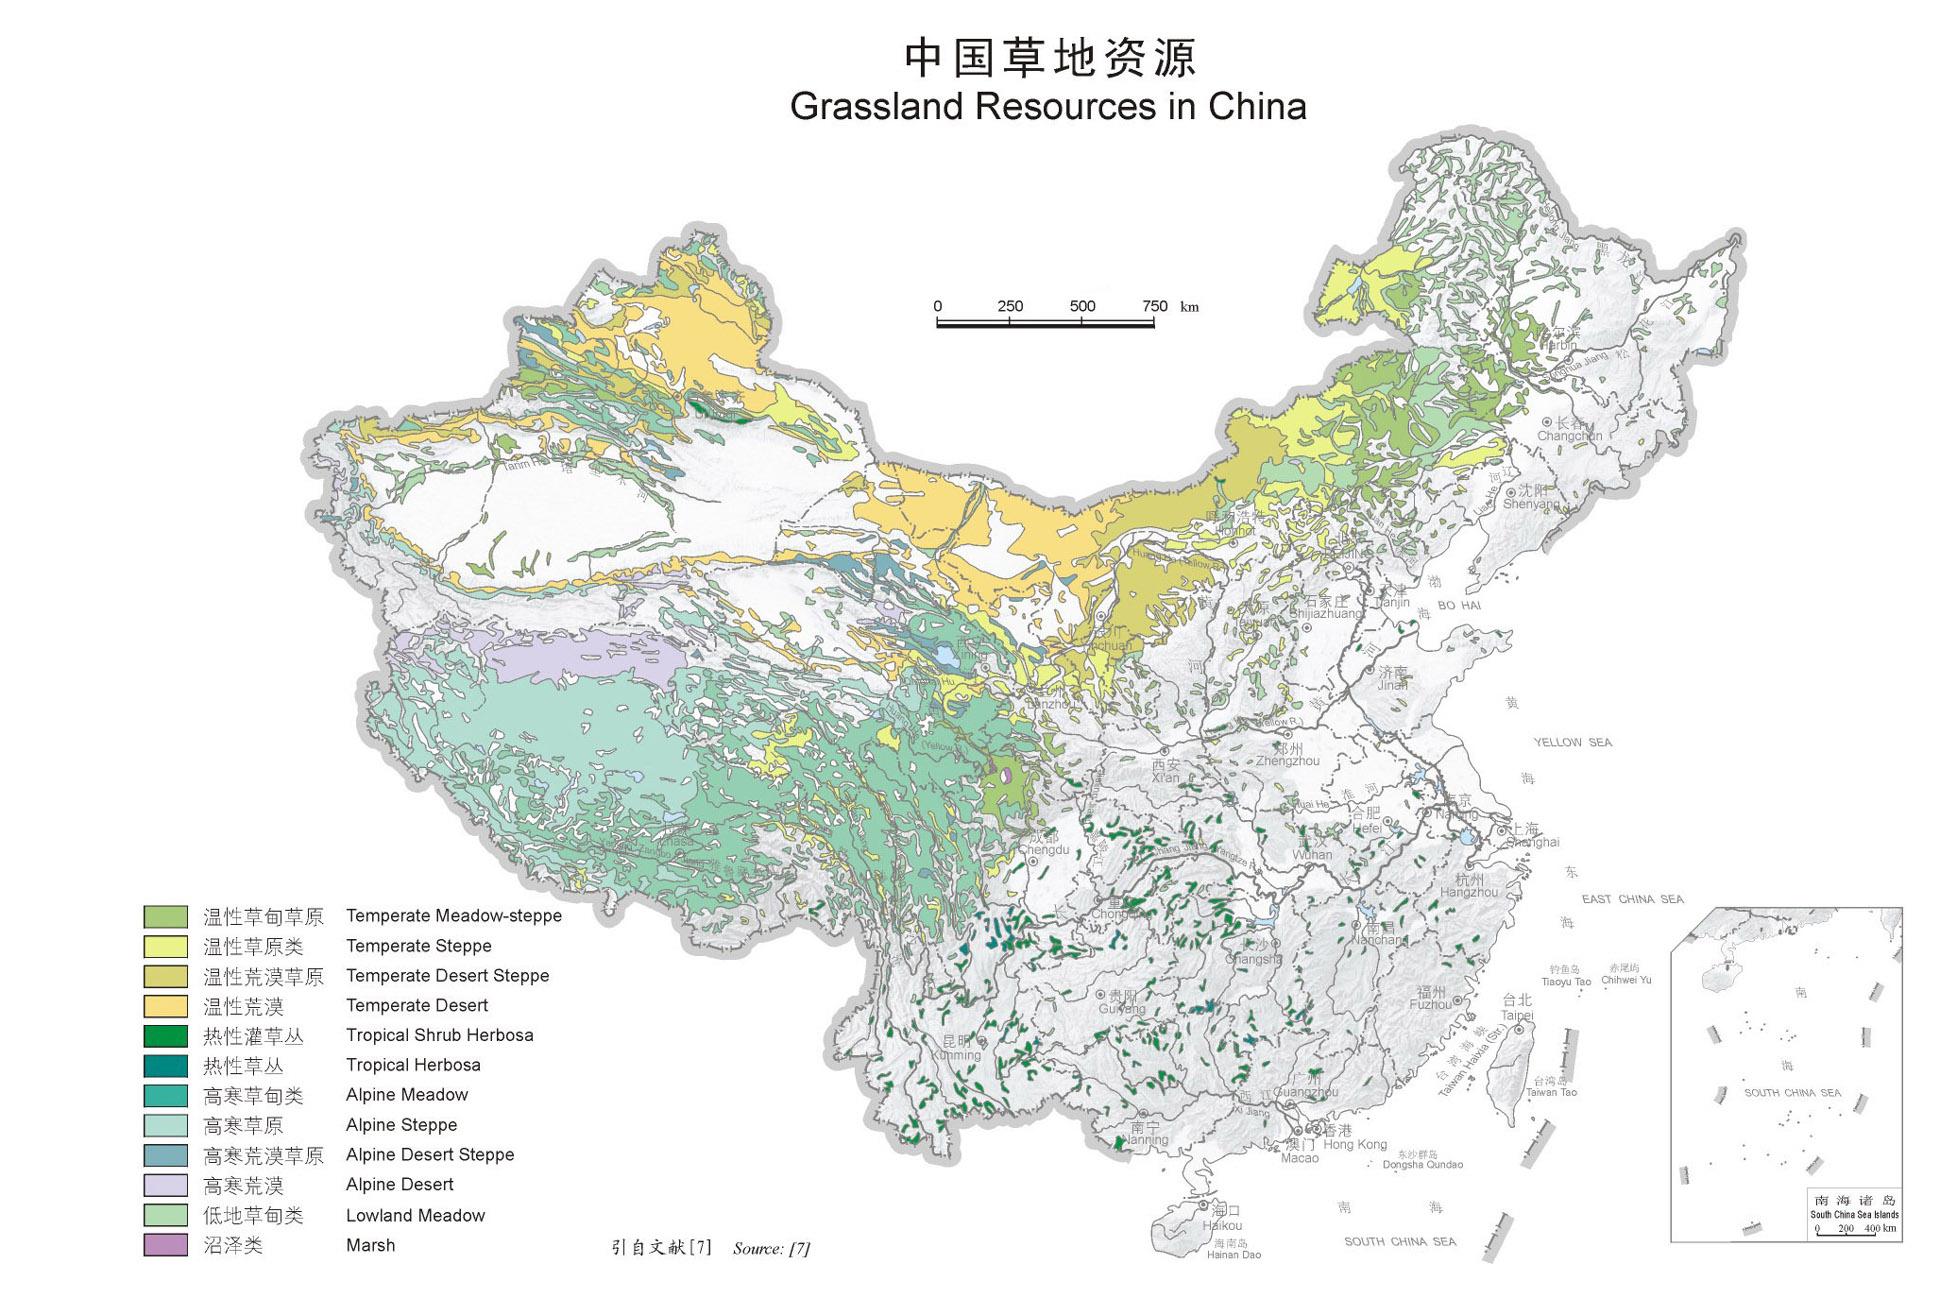
\includegraphics[width = 0.9\textwidth]{./pic/1.1.1.jpg}
		\end{center}
		%\vspace{15mm}
		\only<6>{
		我国是世界上第二大草地资源大国,天然草原面积3.94×108hm2,约占我国国土面积的41.7\%,是耕地面积的3 倍左右,林地面积的2 倍多(刘黎明,2002)。
	    }
		\column{0.3\textwidth}
		主要分布					
		\begin{itemize}
			\item<1-> 东北平原
			\item<2-> 内蒙古高原
			\item<3-> 黄土高原
			\item<4-> 青藏高原
			\item<5-> 新疆山地
		\end{itemize}
	\end{columns}
\end{frame}

\subsection{研究现状}
\begin{frame}{\insertsubsection}
	\begin{center}
		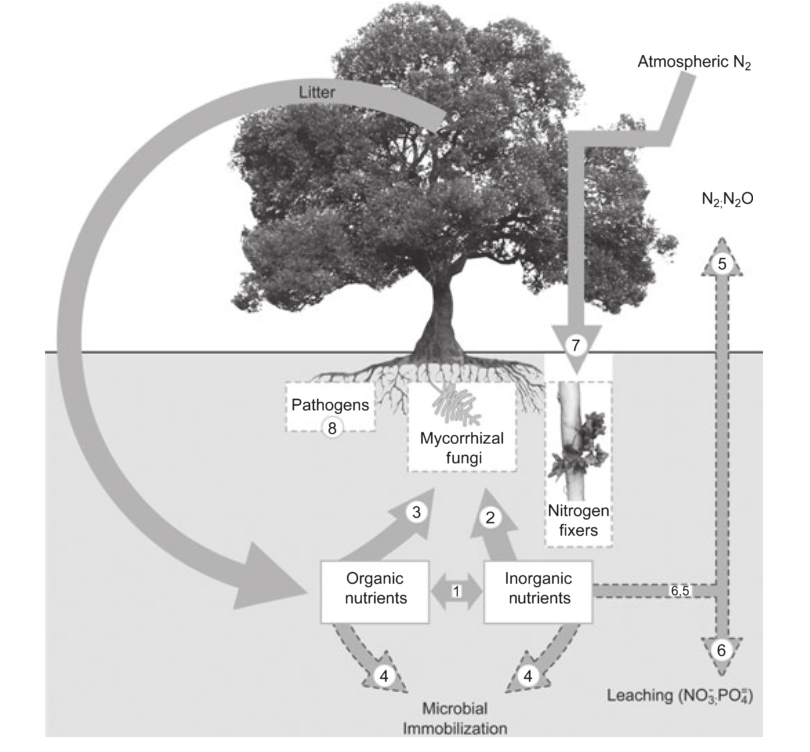
\includegraphics[width = 0.9\textwidth]{./pic/1.1.2.jpg}
	\end{center}
\end{frame}
\begin{frame}{\insertsubsection}
	\begin{columns}
		\column{0.5\textwidth}
		植物物种多样性与微生物多样性的关系	
		\begin{center}
			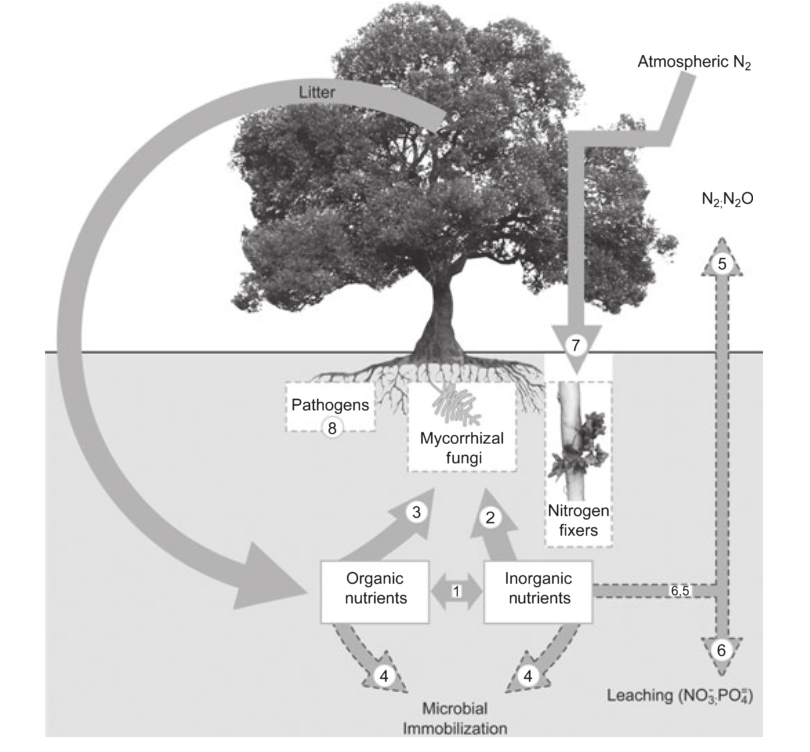
\includegraphics[width = 0.9\textwidth]{./pic/1.1.2.jpg}
		\end{center}
		
		\column{0.5\textwidth}
		植物多样性通过几个方面对微生物产生直接或间接影响:
		\begin{itemize}
			\item<1-> 提高净初级生产力(NPP)
			\item<2-> 提高凋落物的多样性
			\item<3-> 提高食物资源和生境的多样性
			\item<4-> 改变凋落物的质量(C/N)
			\item<5-> 根分泌物的多样性
			\item<6-> 土壤温度、湿度、pH
		\end{itemize}
	\end{columns}
\end{frame}
\begin{frame}{\insertsubsection}
	\begin{center}
		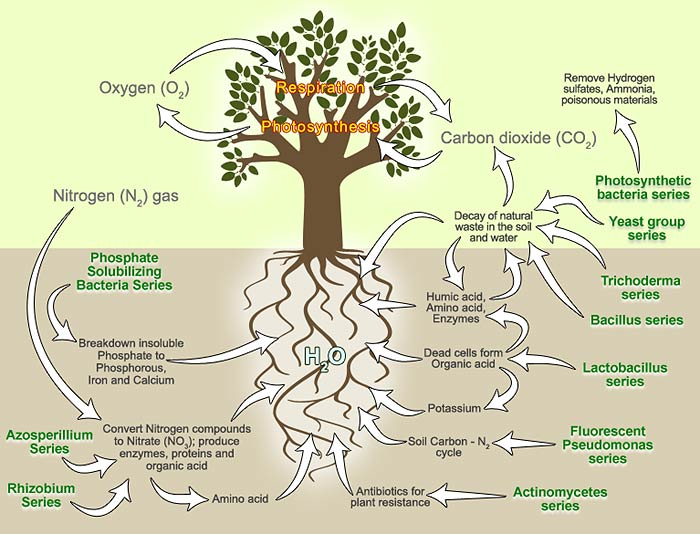
\includegraphics[width = 0.9\textwidth]{./pic/1.1.3.jpg}
	\end{center}
\end{frame}
\begin{frame}{\insertsubsection}
	\begin{columns}
		\column{0.5\textwidth}
		地下微生物群落	
		\begin{center}
			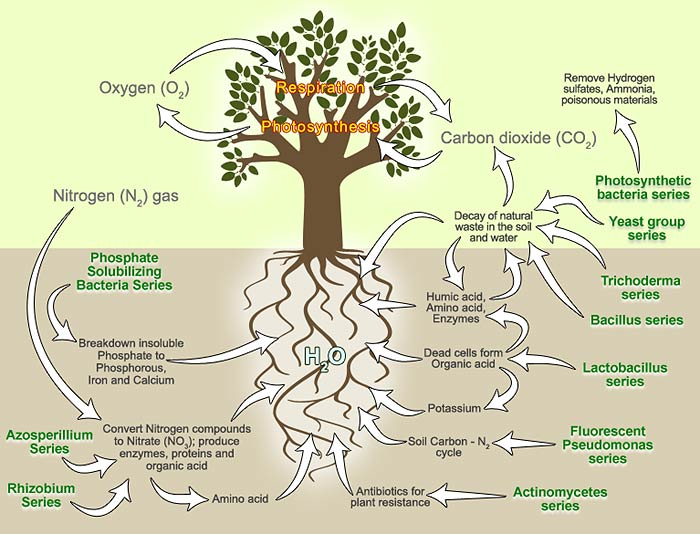
\includegraphics[width = 0.9\textwidth]{./pic/1.1.3.jpg}
		\end{center}
		
		\column{0.5\textwidth}
		地下微生物群落在决定植物群落生产力、多样性和组成中发挥着重要作用(Kulmatiski et al., 2011)。前人的研究结果表明,地下微生物多样性会影响植物生长和生产力、有效养分、生态系统功能。还有一些研究显示微生物群落组成的变化会反馈植物的协同生存(Reynolds et al., 2003)和群落组成(Bever, 2003)。
	\end{columns}
\end{frame}
\subsection{研究现状}
\begin{frame}{\insertsubsection}
	植物物种多样性与微生物多样性的关系
	\begin{center}
		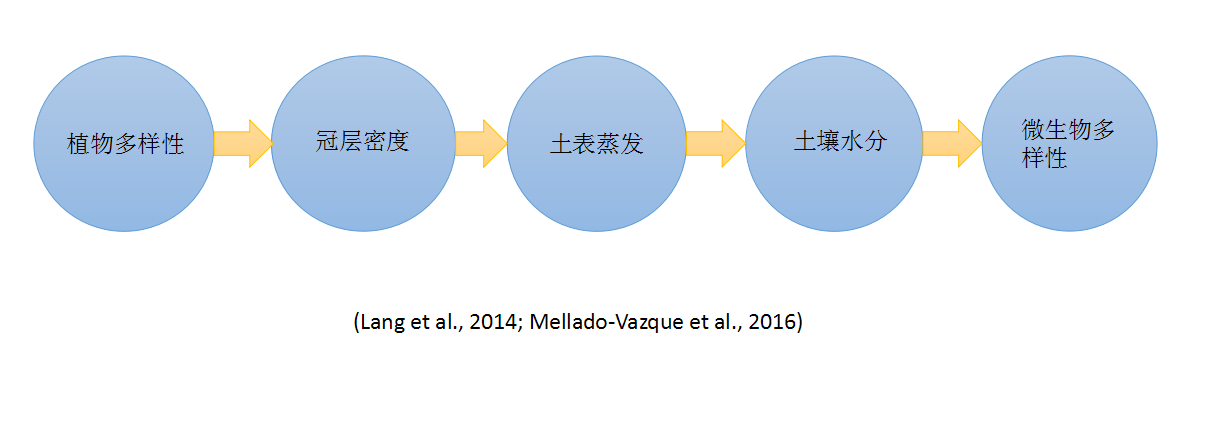
\includegraphics[width = 0.9\textwidth]{./pic/1.2.1.png}
	\end{center}
	这种影响甚至超过土壤质地对微生物的影响
\end{frame}
\begin{frame}{\insertsubsection}
	植物物种多样性与微生物多样性的关系
	\begin{center}
		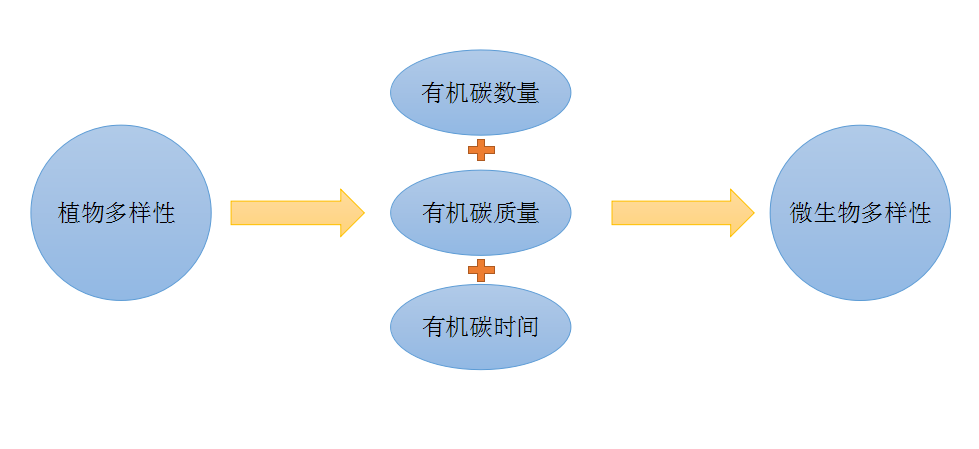
\includegraphics[width = 0.9\textwidth]{./pic/1.2.2.png}
	\end{center}
	(Stephan et al., 2000; Zak et al., 2003; Lange et al., 2014; Weidner et al., 2015; Mellado-Vazque et al., 2016)
\end{frame}
\begin{frame}{\insertsubsection}
	植物物种多样性与微生物多样性的关系
	微生物对植物的影响
		\begin{center}
			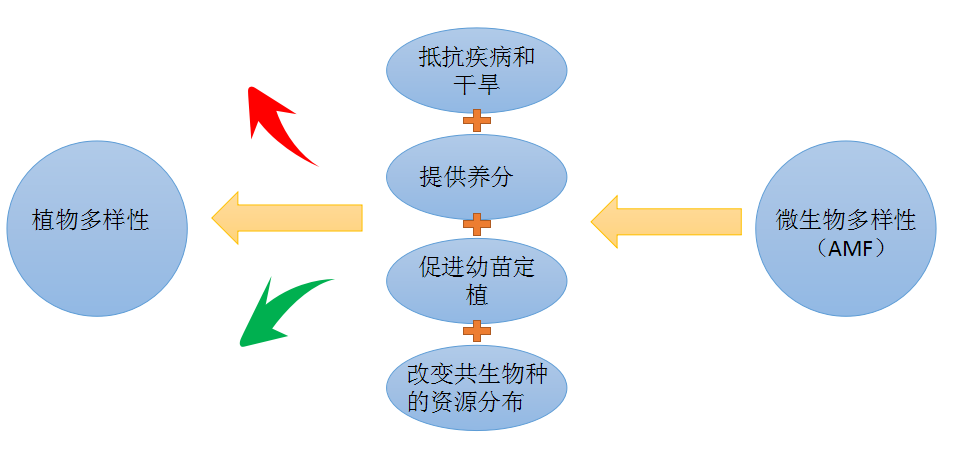
\includegraphics[width = 0.9\textwidth]{./pic/1.2.3.png}
		\end{center}
		(Van der Heijden et al., 1998; Hartnett \&  Wilson, 1999; O'Connor et al., 2002; Van der Heijden et al., 2006; Sikes et al., 2009; Schnitzer et al., 2011; )
\end{frame}
\begin{frame}{\insertsubsection}
	植物物种多样性与微生物多样性的关系
	\begin{center}
		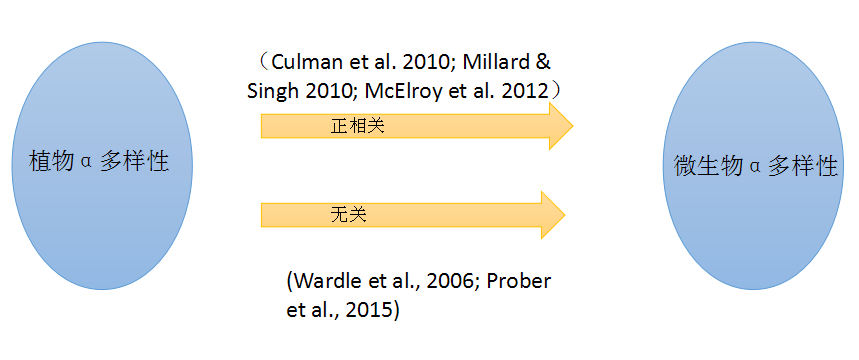
\includegraphics[width = 0.9\textwidth]{./pic/1.2.4.png}
	\end{center}
\end{frame}

\begin{frame}{\insertsubsection}
	植物功能群多样性对微生物多样性的关系
		\begin{center}
			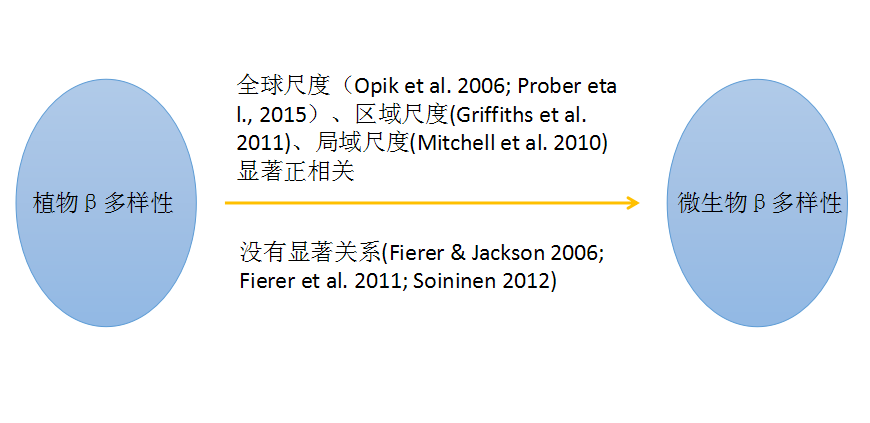
\includegraphics[width = 0.9\textwidth]{./pic/1.2.5.png}
		\end{center}
\end{frame}


\subsection{研究目的}
\begin{frame}{\insertsubsection}
	研究目的
	\begin{itemize}
		\item 沿水分梯度条件下,高寒草地和温性草地植物物种多样性和微生物多样性的关系
		\item 沿水分梯度条件下,高寒草地和温性草地植物功能群多样性与微生物多样性的关系
		\item 在不同生态系统类型条件下,植物物种多样性和功能群多样性对微生物多样性的影响
	\end{itemize}
\end{frame}